\thispagestyle{cackithitoannone}
\pagestyle{cackithitoan}
\everymath{\color{cackithi}}
\graphicspath{{../cackithi/pic/}}
\begingroup
\AddToShipoutPicture*{\put(0,616){
\includegraphics[width=19.3cm]{../bannercackithi}}}
\AddToShipoutPicture*{\put(110,527){
\includegraphics[scale=1]{../tieude.pdf}}}
\centering
\endgroup
\vspace*{182pt}

\begin{multicols}{2}
	\textbf{\color{cackithi}Vài nét về kỳ thi}
	\vskip 0.1cm 
	Kỳ thi Olympic Toán được tổ chức lần đầu tiên vào năm $2000$ bởi bộ giáo dục đào tạo Pháp và hiệp hội Animath. Đây là kỳ thi dành cho những học sinh lớp $11$ đang theo học tại chương trình Toán của Pháp cả trong và ngoài nước, nhằm mục đích phát triển sự tò mò, khả năng tìm tòi cũng như tư duy phê phán của học sinh thông qua việc xử lý hoặc cá nhân hoặc theo nhóm một số bài toán cụ thể. Bên cạnh đó, kỳ thi còn nhằm phát triển và nâng cao văn hóa khoa học và công nghệ, nhằm mục đích kích thích sự sáng tạo và chủ động của học sinh, khơi dậy trong học sinh niềm yêu thích với bộ môn Toán đặc biệt khích lệ các bạn nữ mạnh dạn hướng tới việc nghiên cứu khoa học. Kỳ thi cho phép học sinh tiếp cận các vấn đề Toán học theo cách mở đầy hứng thú thông qua những ví dụ nhấn mạnh mối liên hệ giữa Toán và các ngành khoa học khác. Chính vì vậy kỳ thi được tổ chức dựa trên tinh thần tự nguyện của học sinh và nội dung của đề thi chỉ gói gọn trong chương trình Toán cấp $2$, lớp $10$ và lớp $11$. 
	\vskip 0.1cm
	Bắt đầu từ tháng $2$ hàng năm, giáo viên bộ môn Toán lớp $11$ sẽ đại diện đăng ký tham gia cho học sinh qua trang web của Sở giáo dục. Kỳ thi Olympic Toán lần thứ $23$ tại Pháp đã diễn ra vào thứ $4$ ngày $15$ tháng $03$ năm $2023$, được tổ chức bởi chính các giáo viên bộ môn Toán và tại những trường có học sinh tham gia kỳ thi. Học sinh trải qua hai bài thi độc lập, mỗi bài thi kéo dài $120$ phút trong cùng một ngày. 
	\begin{figure}[H]
		\vspace*{-10pt}
		\centering
		\captionsetup{labelformat= empty, justification=centering}
		
\includegraphics[width= 1\linewidth]{1}
%		\caption{\small\textit{\color{}.}}
		\vspace*{-15pt}
	\end{figure}
	Bài thi thứ nhất là bài thi cấp quốc gia bao gồm ba bài tập. Học sinh tham gia bài thi cấp quốc gia theo hình thức thi cá nhân. Mỗi học sinh tùy theo chương trình học chuyên hay không chuyên sẽ chọn hai trong ba bài tập trong đề thi, trong đó bài $1$ dành chung cho tất cả các thí sinh, bài $2$ dành cho các thí sinh theo chương trình chuyên, bài $3$ dành cho các thí sinh không theo chương trình chuyên. 
	\vskip 0.1cm
	Bài thi số hai là bài thi cấp tỉnh bao gồm hai bài tập và điểm đặc biệt của bài thi này là học sinh có thể chọn hoặc thi cá nhân hoặc thi theo nhóm từ $2$ tới $3$ thí sinh thậm chí các thành viên trong nhóm có thể tới từ những lớp khác nhau trong cùng một khối và đặc khuyến khích những nhóm có sự tham gia của cả nam và nữ nhằm mục đích cổ vũ và phát huy khả năng làm việc nhóm của từng học sinh. 
	\vskip 0.1cm
	Hội đồng chấm thi được chỉ định và cũng được chia thành hai cấp: quốc gia và cấp tỉnh. Trong đó hội đồng cấp tỉnh một mặt chấm bài thi cấp tỉnh của các thí sinh ở tỉnh đó nhằm chọn ra những bài làm xuất sắc nhất để trao huy chương, bên cạnh đó còn chọn lựa từ những bài thi cấp quốc gia của tỉnh mình những bài làm xuất sắc nhất để gửi lên hội đồng cấp quốc gia. Qua đó, hội đồng cấp quốc gia xem xét và chọn ra trong những đề cử từ các tỉnh khác nhau những bài làm xuất sắc nhất để trao huy chương. 
	\vskip 0.1cm
	Dưới sự tài trợ của hiệp hội Animath, viện nghiên cứu tin học và tự động  INRIA, Texas instrument, Casio, Ecole Polytechnique…những học sinh đạt giải cấp quốc gia cùng gia đình và giáo viên Toán đã được mời tham dự lễ tổng kết trao giải đã diễn ra vào ngày $07.06.2023$ tại Viện nghiên cứu về thế giới Ả rập, Paris. Qua đó, học sinh có cơ hội để tìm hiểu về lịch sử của kỳ thi Olympic Toán, gặp gỡ những nhà Toán học hàng đầu như và nghe báo cáo của các giáo sư và nghiên cứu sinh đang nghiên cứu về Toán. Đặc biệt hơn, những thí sinh có kết quả xuất sắc sẽ được cấp học bổng có cơ hội tham gia vào các trường hè cũng như những khóa thực tập để chuẩn bị cho những kỳ thi Olympic Toán khác ...
	\vskip 0.1cm
	\centerline{\textbf{\color{cackithi}Đề thi Olympic Toán lần thứ $\pmb{23.}$}}
	\vskip 0.1cm
	 \textbf{\color{cackithi}Phần $\pmb{1}$: Đề thi Olympic Toán cấp quốc gia năm $\pmb{2023.}$}
	\vskip 0.1cm
	 \textbf{\color{cackithi}Bài $\pmb{1}$ ( Chung cho tất cả thí sinh).}
	\vskip 0.1cm 
	\centerline{ \textbf{\color{cackithi}Mạnh hơn nữa!}}
	\vskip 0.1cm
	Một người chơi tráo bộ bài gồm $n$ quân bài được đánh số từ $1$ tới $n$, trong đó $n$ là số tự nhiên lớn hơn hoặc bằng $3$. Sau khi trộn đều, người chơi ghi lại thứ tự từng quân bài nhận được. Ta gọi những số nhận được đó là một \textit{liste}.
	\vskip 0.1cm 
	Số tự nhiên $n$ được gọi là chiều dài của \textit{liste}. Ví dụ trường hợp $n=8$, một trong những \textit{liste} có thể nhận được là $L=[2,5,7,6,1,8,4,3]$.
	\vskip 0.1cm 
	Với một \textit{liste} cho trước, người chơi ghi được một điểm khi số của một quân bài trong \textit{liste} lớn hơn số của quân bài nằm liền kề trước nó. Ví dụ với liste $L=[2,5,7,6,1,8,4,3]$, người chơi ghi được $3$ điểm. 
	\vskip 0.1cm
	Ta gọi \textit{score} là số điểm được ghi bởi người chơi. Ở ví dụ trên, \textit{score} của người chơi là $3$.
	\vskip 0.1cm 
	$\pmb{1.}$ \textit{Một vài ví dụ}
	\vskip 0.1cm 
	$a)$ Hãy cho một ví dụ khác về một \textit{liste} với chiều dài $8$ và \textit{score} $3$.
	\vskip 0.1cm 
	$b)$ Hãy tìm tất cả các \textit{liste} có chiều dài $n=3$ và xác định \textit{score} tương ứng. 
	\vskip 0.1cm
	Trở lại trường hợp $n$ tổng quát. 
	\vskip 0.1cm
	$2.$ Hãy viết một hàm bằng ngôn ngữ Python phụ thuộc vào hai tham số \textit{liste} $L$ và chiều dài $n$ của \textit{liste} $L$. Biết rằng hàm đó cho ra kết quả là \textit{score} của \textit{liste} $L$. 
	\vskip 0.1cm
	$3.$ Chứng minh rằng \textit{score} là số tự nhiên lớn hơn hoặc bằng $0$, nhỏ hơn hoặc bằng $n-1$. Hãy tìm một \textit{liste} mà ở đó \textit{score} bằng $0$ và một \textit{liste} mà ở đó \textit{score} bằng $n-1$.
	\vskip 0.1cm 
	$4.$ Xét $k$ là số tự nhiên lớn hơn hoặc bằng $1$ và nhỏ hơn hoặc bằng $n-2$.
	\vskip 0.1cm 
	$a)$ Chứng minh rằng tồn tại một \textit{liste} có chiều dài $n$ và có \textit{score} bằng $k$.
	\vskip 0.1cm 
	$b)$ Có thể tìm được hai \textit{liste} có chiều dài $n$ và có \textit{score} bằng $k$ hay không?
	\vskip 0.1cm 
	Ta ký hiệu $L_n(s)$ là số những \textit{liste} có chiều dài $n$ và có \textit{score} bằng $s$.
	\vskip 0.1cm 
	$5.$ Xác định $L_n(0)$ và $L_n (n-1)$.
	\vskip 0.1cm 
	$6.$ Công thức hồi quy.
	\vskip 0.1cm
	$a)$ Hãy tính giá trị $L_3 (0)$, $L_3 (1)$ và $L_3 (2)$. Hãy nêu cách chèn vào I $[3,1,2]$ quân bài mang số $4$ để nhận được một \textit{liste} mới có \textit{score} bằng $1$.
	\vskip 0.1cm 
	$b)$ Hãy nêu cách chèn vào \textit{liste} $[3,2,1]$ quân bài mang số $4$ để nhận được một \textit{liste} mới có \textit{score} bằng $0$.
	\vskip 0.1cm
	$c)$ Hãy kiểm tra đẳng thức $L_4 (1)=2L_3 (1)+3L_3 (0)$.
	\vskip 0.1cm
	$d)$ Chứng minh rằng với mọi số tự nhiên $n\ge3$, ta có:
	\begin{align*}
		L_(n+1) (1)=2L_n (1)+3L_n (0).
	\end{align*}
	$e)$ Với mỗi số tự nhiên $n\ge3$ và số tự nhiên $k\ge1$, biểu diễn $L_(n+1) (k)$ dựa vào $L_n (k)$ và $L_n (k-1)$.
	\vskip 0.1cm 
	Xác định bảng giá trị của $L_n (k)$ tương ứng với $n \in \{3,4,5\}$ và $k \in \{0,1,2,3,4\}$.
	\vskip 0.1cm 
	 \textbf{\color{cackithi}Bài $\pmb{2}$ ( Dành cho những thí sinh hệ phổ thông phổ quát theo chương trình chuyên).}
	\vskip 0.1cm 
	\centerline{ \textbf{\color{cackithi}Giảm vô hạn!}}
	\vskip 0.1cm 
	Gọi  $\alpha$ là số tự nhiên lớn hơn hoặc bằng $4$. Ta xét phương trình $(E)$ dưới đây với ẩn là bộ ba số nguyên $(x_1,x_2,x_3 ) \in \mathbb{Z}^3$.
	\begin{align*}
		(E): x_1^2+x_2^2+x_3^2= \alpha x_1x_2x_3.
	\end{align*}
	Mục đích của bài tập này là chứng minh rằng nghiệm nguyên duy nhất của phương trình $(E)$ là bộ ba $(0,0,0)$. 
	\vskip 0.1cm
	 \textbf{\color{cackithi}Phần $\pmb{1}$.} 
	\vskip 0.1cm
	Với hai số thực $b,c$ cho trước, ta xét hàm số $P$ được định nghĩa từ $\mathbb{R}$ vào $\mathbb{R}$ bởi công thức $P(x)=x^2+bx+c$. Số thực $r$ được gọi là nghiệm của $P$ nếu như $P(r)=0$. Trong phần này, ta giả sử rằng $P$ có hai nghiệm phân biệt $r_1$ và $r_2$. Ta suy ra rằng $P(x)=(x-r_1)(x-r_2)$, với mọi số thực $x$.
	\vskip 0.1cm 
	$1.$ Biểu diễn $b$ và $c$ theo nghiệm $r_1$ và $r_2$.
	\vskip 0.1cm
	$2.$ Giả sử rằng $b\le 0$ và $c\ge0$. Ta có thể nói gì về dấu của các nghiệm $r_1$ và $r_2$?
	\vskip 0.1cm 
	 \textbf{\color{cackithi}Phần $\pmb{2}$.}
	\vskip 0.1cm
	$1a)$. Giả sử rằng bộ ba $(x_1,x_2,x_3 ) \in \mathbb{Z}^3$ là nghiệm của phương trình $(E)$. Chứng minh rằng bộ ba ($|x_1 |,|x_2 |,|x_3 |$) cũng là nghiệm của phương trình $(E)$.
	\vskip 0.1cm
	$1b)$. Từ đó suy ra rằng, nếu tồn tại một bộ ba số nguyên khác $(0,0,0)$ là nghiệm của phương trình $(E)$ thì tồn tại một bộ ba số tự nhiên khác $(0,0,0)$ là nghiệm của phương trình $(E)$.
	\vskip 0.1cm 
	$2.$ Nếu bộ ba $(x_1,x_2,x_3 ) \in \mathbb{Z}^3$ là nghiệm của phương trình $(E)$, ta có thể nói gì về bộ ba số nguyên $(x_2,x_1,x_3)$?
	\vskip 0.1cm 
	$3.$ Từ đó suy ra rằng nếu phương trình $(E)$ có nghiệm khác $(0,0,0)$ trong $\mathbb{Z}^3$ thì cũng có nghiệm $(x_1,x_2,x_3)$ trong $\mathbb{N}^3$ khác $(0,0,0)$ sao cho $x_1 \le x_2 \le x_3$.
	\vskip 0.1cm 
	 \textbf{\color{cackithi}Phần $\pmb{3.}$}
	\vskip 0.1cm
	Trong phần này, ta giả sử tồn tại một bộ ba số tự nhiên $(x_1,x_2,x_3)$ khác $(0,0,0)$ là nghiệm của phương trình $(E)$ thỏa mãn $x_1 \le x_2 \le x_3$. Ta cố định bộ ba $(x_1,x_2,x_3)$.
	\vskip 0.1cm 
	$1.$ Chứng minh rằng $x_1>0$.
	\vskip 0.1cm
	$2.$ Gọi $Q$ là hàm số được định nghĩa từ $\mathbb{R}$ vào $\mathbb{R}$ bởi công thức $Q(x)=x^2- \alpha x_1 x_2 x+x_1^2+x_2^2$. Một số thực $r$ thỏa mãn $Q(r)=0$ được gọi là nghiệm của $Q$.
	\vskip 0.1cm 
	$a)$ Với $y$ là một số thực. Chứng minh rằng bộ ba $(x_1,x_2,y)$ là nghiệm của phương trình $(E)$, khi và chỉ khi, $y$ là nghiệm của $Q$.
	\vskip 0.1cm
	$b)$ Dựa vào đề bài, hãy chỉ ra một nghiệm của $Q$.
	\vskip 0.1cm
	$c)$ Kiểm tra rằng $Q(x_2 )=(3- \alpha x_1 )x_2^2+x_1^2-x_2^2$, từ đó suy ra rằng $Q(x_2 )<0$.
	\vskip 0.1cm 
	$d)$ Dấu của $Q(0)$ là gì?
	\vskip 0.1cm 
	$e)$ Chứng minh rằng $Q$ có hai nghiệm phân biệt: một nghiệm cho ở ý $b)$, một nghiệm ký hiệu là $y$. Hãy sắp xếp những số $0,x_2,x_3$ và $y$ theo thứ tự tăng dần và chứng minh rằng những số đó đôi một khác nhau. 
	\vskip 0.1cm
	$f)$ Chứng minh rằng $(x_1,x_2,y)$ là bộ ba những số tự nhiên thỏa mãn phương trình $(E)$.
	\vskip 0.1cm 
	$3.$ Bằng cách lặp lại quá trình ở phần $3)$ ý $2)$ với bộ ba gồm $x_1,x_2,y$ được xếp theo thứ tự tăng dần thay vì bộ ba $(x_1,x_2,x_3)$, ta nhận được điều gì?
	\vskip 0.1cm
	$4.$ Từ những kết quả trên, hãy suy ra điều vô lý, từ đó kết luận về nghiệm nguyên của phương trình $(E)$.
	\vskip 0.1cm
	$5.$ Chứng minh kết quả sau: ``Với mọi $n \in \mathbb{N}$ và  $\alpha \in \mathbb{N}$ sao cho  $\alpha>n\ge2$. Phương trình $x_1^2+x_2^2+⋯+x_n^2= \alpha x_1 x_2\ldots x_n$  với ẩn số là bộ gồm $n$ số $(x_1,x_2,\ldots,x_n)$ không có nghiệm nguyên nào khác ngoài bộ n số $(0,0,\ldots,0)$". 
	\vskip 0.1cm
	 \textbf{\color{cackithi}Bài $\pmb{3}$ (Dành cho những thí sinh hệ phổ thông phổ quát không theo chương trình chuyên).} 
	\vskip 0.1cm
	\centerline{ \textbf{\color{cackithi}Mã dò và Mã hiệu chỉnh!}}
	\vskip 0.1cm 
	 \textbf{\color{cackithi}Một vài câu hỏi sơ bộ.}
	\vskip 0.1cm
	$1.$ Xét hai số tự nhiên $a,b$. Chứng minh rằng tổng $a+b$ là một số tự nhiên chẵn khi và chỉ khi $a$ và $b$ cùng tính chẵn lẻ. 
	\vskip 0.1cm
	 \textbf{\color{cackithi}Mã hóa một tin nhắn.}
	\vskip 0.1cm
	Một tin nhắn trong bài tập này là một số $M$ được mã hóa thông qua bộ bốn $(x_1,x_2,x_3,x_4)$ với $x_1,x_2,x_3 $ và $ x_4$ là những ``bits", tức là những số chỉ nhận giá trị hoặc $0$ hoặc $1$. Số $M$ biểu diễn thông qua bộ bốn $(x_1,x_2,x_3,x_4)$ được gọi là \textit{nửa -- octet} của thông tin và được định nghĩa bởi: 
	\begin{align*}
		M=x_1+2x_2+4x_3+8x_4.
	\end{align*}
	Ví dụ bộ bốn $(0,0,1,1)$ biểu diễn cho số $M=12$ bởi vì $0+2 \times 0+4×1+8 \times 1=12$. 
	\vskip 0.1cm
	$2a)$. Hãy tìm tin nhắn $M$ được mã hóa bởi bộ bốn $(1,0,0,1)$.
	\vskip 0.1cm
	$2b)$. Hãy tìm một mã hóa của tin nhắn $M=10$. Câu hỏi tương tự với $M=15$.
	\vskip 0.1cm
	$2c)$. Tồn tại hay không một mã hóa của tin nhắn $M=20$? 
	\vskip 0.1cm
	$2d)$. Hãy tìm tất cả các tin nhắn $M$ có thể mã hóa được thông qua bộ bốn được định nghĩa ở trên. 
	\vskip 0.1cm
	\textit{Đôi khi những tin nhắn bị sai lệch so với bản gốc( hay còn gọi là ``bị hỏng") trong quá trình truyền do phần cứng bị lỗi hoặc do những tín hiệu giả. Các lỗi thường thay đổi các ``bits", tức là $0$ chuyển thành $1$ hoặc $1$ chuyển thành $0$. Do đó các kỹ thuật để phát hiện cũng như để sửa chữa những bất thường như thế đã được phát triển. Đó cũng là mục đích được đề cập trong những phần tiếp theo của bài tập này.}
	\vskip 0.1cm
	 \textbf{\color{cackithi}Mã hóa một tin nhắn với sự bảo vệ lỗi.}
	\vskip 0.1cm 
	$\pmb{3.}$  \textbf{\color{cackithi}Nguyên tắc bit chẵn lẻ.}
	\vskip 0.1cm 
	Bộ bốn mã hóa $(x_1,x_2,x_3,x_4)$ được chuyển thành bộ năm mã hóa $(x_1,x_2,x_3,x_4,y)$, trong đó bit $y$ phụ thuộc vào tính chẵn lẻ, cụ thể hơn $y=0$ nếu như tổng $x_1+x_2+x_3+x_4$ chẵn và $y=1$ nếu như tổng đó là lẻ. Ta gọi $y$ là bit chẵn lẻ. Chính bộ năm này sẽ được truyền đi và nó đại diện cho cùng một tin nhắn  $M=x_1+2x_2+4x_3+8x_4$ tương ứng với mã hóa $(x_1,x_2,x_3,x_4)$. Lưu ý rằng các bit chứa thông tin chính $x_1,x_2,x_3,x_4$ và bit chẵn lẻ $y$ được truyền đi một cách thận trọng.
	\vskip 0.1cm 
	Ta xét ví dụ về tin nhắn $M=12$ được mã hóa bởi bộ bốn $(0,0,1,1)$, ở đây $x_1+x_2+x_3+x_4=0+0+1+1=2$ là một số chẵn nên $y=0$. Thay vì truyền đi bộ bốn $(0,0,1,1)$ thì ta truyền đi bộ năm $(0,0,1,1,0)$. 
	\vskip 0.1cm
	$a)$ Hãy xác định bit chẳn lẻ $y$ liên kết với bộ bốn $(1,0,0,1)$ mã hóa cho tin nhắn $M=9$.
	\vskip 0.1cm 
	$b)$ Sau khi tin nhắn mã hóa được truyền đi, ta nhận được bộ năm $(1,1,0,1,0)$ với bít chẵn lẻ được xem là đáng tin cậy. Chứng minh rằng thông tin do mã truyền tải đã bị hỏng.
	\vskip 0.1cm 
	$c)$ Nếu ta chắc chắn về độ tin cậy của bit chẵn lẻ, liệu ta có thể phát hiện ra sự sai lệch cũng như phát hiện ra vị trí sai lệch trong những trường hợp sau hay không?
	\vskip 0.1cm 
	$\bullet$ Trong trường hợp chỉ có một bit chứa thông tin bị sai lệch khi được truyền đến?
	\vskip 0.1cm 
	$\bullet$ Trong trường hợp có hai bit chứa thông tin bị sai lệch khi được truyền đến?
	\vskip 0.1cm
	$\pmb{4.}$  \textbf{\color{cackithi}Nguyên tắc bit điều khiển.}
	\vskip 0.1cm 
	Bộ bốn mã hóa $(x_1,x_2,x_3,x_4)$ được chuyển thành bộ bảy mã hóa $(x_1,x_2,x_3,x_4,y_1,y_2,y_3)$ trong đó $y_1=0$ nếu $x_1+x_2+x_3$ chẵn, $y_1=1$ nếu ngược lại, $y_2=0$ nếu $x_2+x_3+x_4$ chẵn, $y_2=1$ nếu ngược lại và  $y_3=0$ nếu $x_1+x_3+x_4$ chẵn, $y_3=1$ nếu ngược lại. Các bit $y_1,y_2,y_3$ được gọi là bit điều khiển. Các bit chứa thông tin chính là $x_1,x_2,x_3,x_4$. Bộ bảy $(x_1,x_2,x_3,x_4,y_1,y_2,y_3)$ vẫn mã hóa cùng một tin nhắn $M=x_1+2x_2+4x_3+8x_4$. 
	\vskip 0.1cm
	$a)$ Hãy xác định các bit điều khiển $y_1,y_2,y_3$ liên kết với bộ bốn $(1,0,0,1)$ mã hóa cho tin nhắn $M=9$.
	\vskip 0.1cm
	$b)$ Tại sao ta chắc chắn rằng bộ bảy nhận được $(1,1,0,1,0,0,1)$ là một sai lệch trong quá trình truyền tin với điều kiện ta chắc chắn về độ tin cậy của các bit điều khiển?
	\vskip 0.1cm 
	$c)$ Giả sử rằng ta chắc chắn về tính chính xác của các bit điều khiển, trong trường hợp có đúng một trong bốn bit chứa thông tin bị sai, tại sao ta có thể phát hiện ra rằng đã có sự sai lệch và tại sao ta có thể xác định ra vị trí cũng như sửa chữa sự sai lệch đó? Liệu chúng ta có thể phát hiện lỗi khi biết rằng có đúng hai trong bốn bit chứa thông tin bị sai hay không? 
	\vskip 0.1cm
	\begin{center}
		 \textbf{\color{cackithi}Phần $\pmb{2}$: Đề thi Olympic Toán cấp tỉnh -- NICE năm $\pmb{2023}$.}
	\end{center} 
	 \textbf{\color{cackithi}Đề thi dành cho những thí sinh theo chương trình chuyên và tham gia dưới hình thức thi theo nhóm.}
	\vskip 0.1cm 
	 \textbf{\color{cackithi}Bài $\pmb{1.}$ Những khối số học.}
	\vskip 0.1cm
	Trong bài tập này, $n$ là một số tự nhiên lớn hơn hoặc bằng $2$.
	\vskip 0.1cm 
	Ta định nghĩa Khối kích thước $n$ là một bảng trắng gồm $n$ dòng và $n$ cột trong đó một số ô được tô màu đen theo nguyên tắc sau: Nếu một ô có màu đen thì ô ở ngay dưới dưới ô đó cũng có màu đen.
	\vskip 0.1cm
	Ở ví dụ dưới đây, hình $1$, hình $2$ và hình $3$ là những Khối khác nhau có kích thước $3$. Còn hình $4$ không phải là một Khối. 
	\begin{figure}[H]
		\vspace*{-5pt}
		\centering
		\captionsetup{labelformat= empty, justification=centering}
		\begin{tikzpicture}[cackithi,scale=0.6,node font= \small]
			\filldraw[gray] (12,4) rectangle (13,5);
			\filldraw[gray] (13,4) rectangle (14,7);
			\filldraw[gray] (9,0) rectangle (10,3);
			\filldraw[gray] (10,0) rectangle (11,1);
			\filldraw[gray] (12,0) rectangle (13,1);
			\filldraw[gray] (13,0) rectangle (14,3);
			\filldraw[gray] (14,1) rectangle (15,2);
			\draw (8,4) grid (11,7);
			\draw (12,4) grid (15,7);
			\draw (8,0) grid (11,3);
			\draw (12,0) grid (15,3);
			\draw (9.5,3.5) node {\textit{Hình} $1$};	
			\draw (13.5,3.5) node {\textit{Hình} $2$};
			\draw (9.5,-0.5) node {\textit{Hình} $3$};
			\draw (13.5,-0.5) node {\textit{Hình} $4$};	
		\end{tikzpicture}
		\vspace*{-15pt}
	\end{figure}
	Lưu ý rằng một khi đã được vẽ, ta không thể đảo ngược một Khối.
	\vskip 0.1cm
	$1.$ Hãy vẽ tất cả những Khối có kích thước $2$.
	\vskip 0.1cm
	$2.$ Có bao nhiêu Khối có kích thước $6$?
	\vskip 0.1cm
	Với mỗi ô trong một Khối kích thước $n$, ta gán số như sau:
	\vskip 0.1cm
	$\bullet$ Nếu ô đó màu trắng ta gán số $1$.
	\vskip 0.1cm
	$\bullet$ Nếu ô đó màu đen ở cột thứ $k$ của Khối thì ta gắn với số nguyên tố đứng ở vị trị thứ $k$ theo thứ tự tăng dần của bảng số nguyên tố. Ví dụ số nguyên tố đầu tiên là $2$, số nguyên tố ở vị trí thứ $2$ là $3$, ở vị trí thứ $3$ là $5$, ở vị trí thứ $4$ là $7 \ldots$
	\vskip 0.1cm
	Với mỗi Khối kích thước $n$, ta liên kết với một số tự nhiên duy nhất $i$ được tính bằng cách nhân tất các những số được gán cho $n^2$ ô ở trong Khối đó. 
	\vskip 0.1cm
	Trong bài tập này, ta ký hiệu $B_{i,n}$ là Khối có kích thước $n$ gán với số tự nhiên $i$ được tính như trên. 
	\vskip 0.1cm
	Ví dụ ở Khối được cho bởi hình $1$ phía trên, ta có $n=3$ và $i=1^9=1$, ta gọi Khối đó là $B_{1,3}$. Tương tự như vậy, đối với Khối cho bởi hình $2$, ta có $n=3$ và $i=1^5 \times 2 \times 3^3=54$ ta được Khối tương ứng là $B_{54,3}$.
	\vskip 0.1cm 
	$3.$ Hãy vẽ Khối $B_{90,3}$ có kích thước $3$ và được gán với số $90$.
	\vskip 0.05cm 
	$4.$ Tồn tại hay không một Khối kích thước $3$ liên kết với số tự nhiên $2500$?
	\vskip 0.05cm 
	$5.$ Xác định số tự nhiên lớn nhất liên kết với Khối kích thước $3$.
	\vskip 0.05cm 
	Ta gọi $i$ và $j$ là hai số tự nhiên liên kết với hai Khối kích thước $n$. Ta nói rằng Khối $B_{i,n}$ nằm khít trên Khối $B_{j,n}$ nếu như tất cả các ô được tô màu đen trên Khối $B_{i,n}$ cũng được tô màu đen trên Khối $B_{j,n}$.
	\vskip 0.05cm 
	Ví dụ dưới đây cho thấy Khối được cho bởi hình $5$ nằm khít trên Khối được cho bởi hình $6$ nhưng không nằm khít trên Khối được cho bởi hình $7$. 
	\begin{figure}[H]
		\vspace*{-5pt}
		\centering
		\captionsetup{labelformat= empty, justification=centering}
		\begin{tikzpicture}[cackithi,scale=0.6,node font= \small]
			\filldraw[gray] (0,0) rectangle (3,1);
			\filldraw[gray] (1,1) rectangle (2,2);
			\filldraw[gray] (4,0) rectangle (7,2);
			\filldraw[gray] (4,2) rectangle (5,3);
			\filldraw[gray] (8,0) rectangle (9,3);
			\filldraw[gray] (9,0) rectangle (11,1);
			\filldraw[gray] (10,1) rectangle (11,2);
			\draw (0,0) grid (3,3);		
			\draw (4,0) grid (7,3);
			\draw (8,0) grid (11,3);	
			\draw (1.5, -0.5) node {\textit{Hình} $5$};
			\draw (5.5, -0.5) node {\textit{Hình} $6$};
			\draw (9.5, -0.5) node {\textit{Hình} $7$};
		\end{tikzpicture}
		\vspace*{-10pt}
	\end{figure}
	$6a)$ Hãy vẽ tất cả những Khối nằm khít trên Khối được cho bởi hình $5$ phía trên. 
	\vskip 0.05cm
	$6b)$ Xác định những số tự nhiên $i$ liên kết với từng Khối được vẽ ở ý $6a)$
	\vskip 0.05cm
	$7.$ Với mỗi số tự nhiên $i$ và $j$ liên kết với hai Khối kích thước $n$.
	\vskip 0.05cm 
	$a)$ Chứng minh rằng nếu Khối $B_{i,n}$ nằm khít trên Khối $B_{j,n}$ thì $i$ là ước của $j$.
	\vskip 0.05cm 
	$b)$ Ngược lại, chứng minh rằng nếu $i$ là ước của $j$ thì Khối $B_{i,n}$ nằm khít trên Khối $B_{j,n}$.
	\vskip 0.05cm 
	$c)$ Tìm số những ước dương của số tự nhiên $i$ tương ứng với Khối kích thước $6$ dưới đây:
	\begin{figure}[H]
		\vspace*{-5pt}
		\centering
		\captionsetup{labelformat= empty, justification=centering}
		\begin{tikzpicture}[cackithi,scale=0.6]
			\filldraw[gray] (0,0) rectangle (1,6);
			\filldraw[gray] (1,0) rectangle (2,4);
			\filldraw[gray] (2,0) rectangle (3,5);
			\filldraw[gray] (3,0) rectangle (4,2);
			\filldraw[gray] (4,0) rectangle (5,6);
			\filldraw[gray] (5,0) rectangle (6,5);
			\draw (0,0) grid (6,6);			
		\end{tikzpicture}
		\vspace*{-10pt}
	\end{figure}
	$d)$ Hãy xác định tất cả những số tự nhiên $i$ liên kết với những Khối kích thước $3$ sao cho số đó có đúng $18$ ước dương.
	\vskip 0.05cm
	$e)$ Có bao nhiêu số tự nhiên $i$ liên kết với những Khối kích thước $3$ sao cho số đó có đúng $5$ ước dương.
	\vskip 0.05cm
	Một Khối được gọi là Khối phản chiếu nếu như nó có ít nhất một trục đối xứng. Ở ví dụ dưới đây, ta thấy Khối hình $8$ là Khối phản chiếu còn ở hình $9$ không phải Khối phản chiếu. 
	\begin{figure}[H]
		\vspace*{-5pt}
		\centering
		\captionsetup{labelformat= empty, justification=centering}
		\begin{tikzpicture}[cackithi,scale=0.6,node font=\small]
			\filldraw[gray] (0,0) rectangle (3,2);
			\filldraw[gray] (1,2) rectangle (2,3);
			\filldraw[gray] (5,0) rectangle (7,2);
			\filldraw[gray] (6,2) rectangle (7,3);
			\draw (0,0) grid (3,3);
			\draw  (4,0) grid (7,3);		
			\draw (1.5, -0.5) node {\textit{Hình} $8$};
			\draw (5.5, -0.5) node {\textit{Hình} $9$};	
		\end{tikzpicture}
		\vspace*{-10pt}
	\end{figure}
	$8.$ Hãy chứng minh tính đúng sai của những mệnh đề sau.
	\vskip 0.05cm
	$a)$ Tồn tại một Khối phản chiếu kích thước $3$ có ít nhất hai trục đối xứng.
	\vskip 0.05cm
	$b)$ Khối $B_{270,3}$ là một Khối phản chiếu.
	\vskip 0.05cm
	$c)$ Tồn tại ít nhất $20$ Khối phản chiếu kích thước $3$.
	\vskip 0.05cm 
	$d)$ Tồn tại một Khối phản chiếu kích thước $3$ liên kết với số tự nhiên có đúng $36$ ước.
	\vskip 0.05cm
	$e)$ Với mỗi số tự nhiên dương $k$, tồn tại một Khối phản chiếu liên kết với số tự nhiên có đúng $k$ ước. 
	\vskip 0.05cm
	 \textbf{\color{cackithi}Bài $\pmb{2.}$ Số xoắn ốc.}
	\vskip 0.05cm
	Bằng cách viết các số tự nhiên dương theo hình xoắn ốc, ta nhận được vô số những vành đồng tâm. 
	\begin{figure}[H]
		\vspace*{-5pt}
		\centering
		\captionsetup{labelformat= empty, justification=centering}
		\def\myNotes{{{73,74,75,76,77,78,79,80,81},{72,43,44,45,46,47,48,49,50},{71,42,21,22,23,24,25,26,51},{70,41,20,7,8,9,10,27,52},{69,40,19,6,1,2,11,28,53},{68,39,18,5,4,3,12,29,54},{67,38,17,16,15,14,13,30,55},{66,37,36,35,34,33,32,31,56},{65,64,63,62,61,60,59,58,57}}} 
		\begin{tikzpicture}[scale=0.6,color=cackithi, node font= \scriptsize]
			\filldraw[cackithi!15] (1.5,1.5) rectangle (8.5,2.5);
			\filldraw[cackithi!15] (1.5,2.5) rectangle (2.5,7.5);
			\filldraw[cackithi!15] (1.5,7.5) rectangle (8.5,8.5);
			\filldraw[cackithi!15] (7.5,2.5) rectangle (8.5,7.5);
			
			\filldraw[cackithi!15] (3.5,3.5) rectangle (6.5,4.5);
			\filldraw[cackithi!15] (3.5,5.5) rectangle (6.5,6.5);
			\filldraw[cackithi!15] (3.5,4.5) rectangle (4.5,5.5);
			\filldraw[cackithi!15] (5.5,4.5) rectangle (6.5,5.5);
			\foreach \x  in {1,2,...,9}
			\foreach \y in {1,2,...,9}
			{	
				\draw (\x,\y) +(-.5,-.5) rectangle ++(.5,.5);
				\begin{scope}[shift={(\x,\y)}]
					\pgfmathtruncatemacro{\r}{\myNotes[\y-1][\x-1]}
					\coordinate (C) at (0,0,0);
					\node (C) {$\r$};
				\end{scope}
			}
		\end{tikzpicture}
		\vspace*{-10pt}
	\end{figure}
	Vành số $1$ gồm những số tự nhiên từ $2$ tới $9$, vành số $2$ gồm những số tự nhiên từ $10$ tới $25$, vành thứ $3$ gồm những số tự nhiên từ $26$ tới $49\ldots$
	\vskip 0.05cm 
	 \textbf{\color{cackithi}Phần A. Từ vành này qua vành khác.}
	\vskip 0.05cm
	Vành $1$ được tạo thành bởi $8$ số tự nhiên dương.
	\vskip 0.05cm
	$1.$ Có bao nhiêu số tự nhiên ở vành $2$?
	\vskip 0.05cm 
	$2.$ Có bao nhiêu số tự nhiên tạo nên vành $3$?
	\vskip 0.05cm
	$3.$ Có bao nhiêu số tự nhiên tạo nên vành $6$?
	\vskip 0.05cm
	Với một số tự nhiên $n$ cố định, có bao nhiêu số tự nhiên tạo nên vành thứ $n$? 
	\vskip 0.05cm
	 \textbf{\color{cackithi}Phần B. Đa thức sinh bởi đường chéo.}
	\vskip 0.05cm
	Ta quan tâm tới dãy số tăng $(u_n )_{n \in \mathbb{N}}$ gồm những số tự nhiên thuộc những vành liền kề của hình xoắn ốc và nằm thẳng hàng theo một đường chéo.
	\vskip 0.05cm
	Hình bên cho ta một ví dụ về một dãy như thế với $u_0=22,u_1=44$ và $u_2=74$.
		\begin{figure}[H]
		\vspace*{-5pt}
		\centering
		\captionsetup{labelformat= empty, justification=centering}
		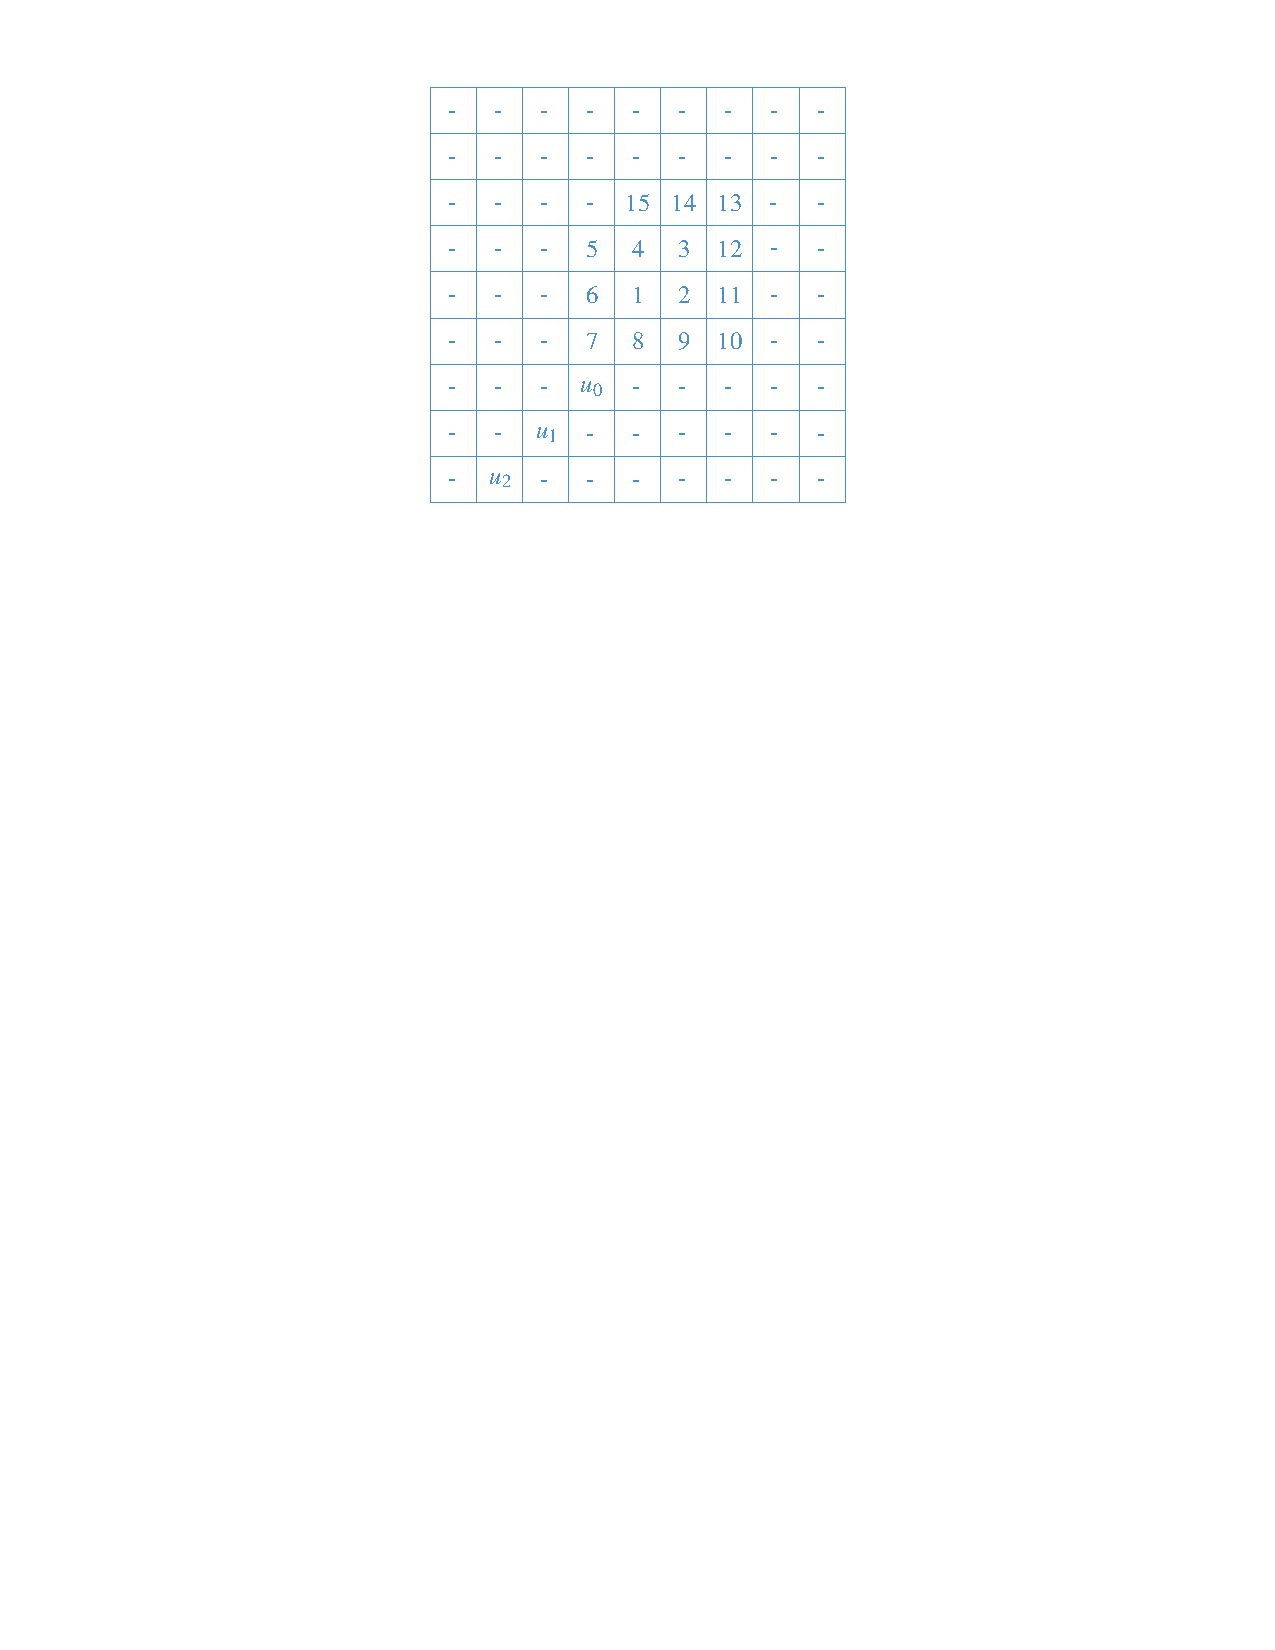
\includegraphics[scale=0.7]{table}
		%		\caption{\small\textit{\color{}.}}
		\vspace*{-12pt}
	\end{figure}	
	Trong phần này ta có thể sử dụng mà không cần phải chứng minh lại công thức tổng của những số tự nhiên từ $1$ tới $n$ sau đây, với $n$ là số tự nhiên dương: 
	\begin{align*}
		1+2+\cdots +n=\dfrac{n(n+1)}{2}.
	\end{align*}
	$\pmb{1.}$  \textbf{\color{cackithi}Đường chéo $\pmb{1.}$}
	\vskip 0.05cm
	Dãy số được được nghĩa với mỗi số tự nhiên $n$ bởi công thức tổng quát $u_n=4n^2+12n+7$ tạo nên một đường chéo của hình xoắn ốc. Trong năm số hạng đầu tiên của dãy $(u_n )_{n \in \mathbb{N}}$, có bao nhiêu số nguyên tố? Giải thích.
	\vskip 0.05cm
	$\pmb{2.}$  \textbf{\color{cackithi}Đường chéo $\pmb{2.}$}
	\vskip 0.05cm
	Xét dãy những số tự nhiên nằm trên đường chéo của hình xoắn ốc theo thứ tự: $u_0=1,u_1=9,u_2=25,u_3=49,u_4=81\ldots$. Không cần chứng minh, với mỗi số tự nhiên $n$, hãy xác định số hạng tổng quát $u_n$ của dãy. 
	\vskip 0.05cm
	$\pmb{3.}$  \textbf{\color{cackithi}Đường chéo $\pmb{3.}$}
	\vskip 0.05cm 
	Xét dãy những số tự nhiên nằm trên đường chéo của hình xoắn ốc theo thứ tự: $u_0=4,u_1=16,u_2=36,u_3=64\ldots$. Ta chấp nhận kết quả rằng tồn tại ba số tự nhiên $a,b,c$ sao cho với mỗi số tự nhiên $n$, số hạng tổng quát $u_n$ của dãy này được viết dưới dạng $u_n=an^2+bn+c$. Hãy xác định giá trị của $a,b,c$.
	\vskip 0.05cm 
	$\pmb{4.}$  \textbf{\color{cackithi}Tổng quát hóa.}
	\vskip 0.05cm 
	Với mỗi số tự nhiên dương $n$, ta đặt $v_n=u_n-u_{n-1}$ và ta chấp nhận kết quả $v_{n+1}=v_n+8$.
	\vskip 0.05cm 
	$a)$ Với mỗi số tự nhiên dương $n$, hãy biểu diễn $v_n$ theo $n$ và $v_1$.
	\vskip 0.05cm
	$b)$ Chứng minh rằng với mỗi số tự nhiên dương $n$, ta có: $u_n-u_0=4n(n-1)+nv_1$.
	\vskip 0.05cm
	$c)$ Từ đó chỉ ra rằng tồn tại hai số tự nhiên $d$ và $e$ sao cho với mỗi số tự nhiên $n$, số hạng tổng quát $u_n$ được cho bởi công thức $u_n=4n^2+dn+e$. Hãy biểu diễn $d$ và $e$ theo $u_0$ và $u_1$.
	\vskip 0.05cm 
	$d)$ Hãy xác định công thức tổng quát của dãy số $u_n$ sinh ra đường chéo của hình xoắn ốc bắt đầu bằng những số nguyên tố: $u_0=5$ và $u_1=19$. Hãy xác định giá trị lớn nhất của $n$ để $u_n$ là số nguyên tố. 
	\vskip 0.05cm
	 \textbf{\color{cackithi}Phần C.  Một vành cho một năm.}
	\vskip 0.05cm
	$1.$ Số tự nhiên $2023$ nằm trên vành thứ bao nhiêu trong hình xoắn ốc? Giải thích. 
	\vskip 0.05cm
	$2.$ Xác định số tự nhiên nhỏ nhất và số tự nhiên lớn nhất của vành được tìm thấy ở ý $1$.
	\vskip 0.05cm 
	 \textbf{\color{cackithi}Tài liệu tham khảo}
	\vskip 0.05cm 
	[$1$] Les sujets et corrigés des olympiades de mathématiques $2023$ | Site pédagogique de Mathématiques (ac-nice.fr).
	\vskip 0.05cm
	[$2$] Les Olympiades nationales de mathématiques | Ministère de l'Education Nationale et de la Jeunesse. 
\end{multicols}
\newpage
\begingroup
\AddToShipoutPicture*{\put(150,690){
\includegraphics[scale=1]{../tieude1.pdf}}}
\centering
\endgroup
\vspace*{20pt}

\begin{multicols}{2}
	Trong phần đầu chuyên mục, chúng tôi sẽ trình bày với các bạn lời giải các bài toán trong trong kỳ thi toán của Đan Mạch mang tên nhà toán học Georg Mohr đăng trong số tháng $4/2023$. 
	\begin{figure}[H]
		\vspace*{-5pt}
		\centering
		\captionsetup{labelformat= empty, justification=centering}
		
\includegraphics[width= 1\linewidth]{gocolympic}
%		\caption{\small\textit{\color{}}}
		\vspace*{-10pt}
	\end{figure}
	{\bf\color{cackithi} OC$\pmb{37.}$} Một con ếch nhảy vào các số nguyên trên trục số. Nếu đang ở một số $n$ chẵn, bước tiếp theo nó sẽ nhảy đến số $\dfrac{n}{2}.$ Nếu đang ở một $n$ số lẻ, nó sẽ nhảy đến số $n + 5$. Tại một thời điểm nó nhảy vào số $25$. Hỏi trước đó $3$ bước nó có thể ở những vị trí nào?
	\vskip 0.1cm
	\textit{Lời giải.} Do $n + 5$ là chẵn nếu $n$ là lẻ nên con ếch luôn nhảy từ một số lẻ đến một số chẵn.
	Vì vậy khi con ếch ở một số lẻ $m$, trước đó một bước nó bắt buộc  phải ở số chẵn $2m.$ Còn  khi
	con ếch ở một số chẵn $m$, trước đó một bước nó có $2$ khả năng: ở số chẵn $2m$ hoặc ở số lẻ $m - 5$.
	\vskip 0.1cm
	Theo lý luận ở trên ta có: khi con ếch ở số $25$, trước đó một bước nó phải ở số $50$. Trước đó $2$ bước, nó phải ở  số $100$ hoặc $45$. 
	Trước đó $3$ bước có $3$ vị trí ếch có thể ở là: $90$, $95$ và $200$.
	\vskip 0.1cm
	{\bf\color{cackithi} OC$\pmb{38.}$} Các số $1, 2, 3, \cdots, 16$  được đặt trong $16$ ô vuông xung quanh một bảng ô vuông cỡ $5\times 5$ như hình bên sao cho tổng của $5$ số trên mỗi cạnh của hình vuông là bằng nhau. 
	Tổng nhỏ nhất có thể có của bốn số trong các ô vuông ở góc là bao nhiêu?
	\begin{figure}[H]
		\vspace*{-5pt}
		\centering
		\captionsetup{labelformat= empty, justification=centering}
		\begin{tikzpicture}[scale=0.9,cackithi]
			\draw (0,0) grid (5,5);
			\draw[fill=white] (1,1) rectangle(4,4);
		\end{tikzpicture}
		\vspace*{-10pt}
	\end{figure}
	\textit{Lời giải.} Đặt $S$ là  tổng của $4$ số ở góc và  $a$ là  tổng của các số trong mỗi hàng, cột của bảng.
	Khi cộng tổng của cả $4$ hàng, cột của bảng lại với nhau, các số ở góc được tính hai lần. Như vậy ta có
	\begin{align*}
		4a = 1 + 2 + . . . + 16 + S.
	\end{align*}
	Ta nhận được $4a = 136 + S$, do đó $S$ phải chia hết cho $4$. Tổng của bốn số nhỏ nhất là $1 + 2 + 3 + 4 = 10$, không chia hết cho $4$. Do $S$ chia hết cho $4$, ta có $S\ge 12$.  Ví dụ sau cho thấy trường hợp $S=12$ có thể xảy ra:
	\begin{figure}[H]
		\vspace*{-5pt}
		\centering
		\captionsetup{labelformat= empty, justification=centering}
		\begin{tikzpicture}[scale=0.9,cackithi]
			\draw (0,0) grid (5,5);
			\draw[fill=white] (1,1) rectangle(4,4);
			\draw (0.5,0.5) node {$6$};
			\draw (1.5,0.5) node {$5$};
			\draw (2.5,0.5) node {$16$};
			\draw (3.5,0.5) node {$9$};
			\draw (4.5,0.5) node {$1$};
			\draw (0.5,4.5) node {$2$};
			\draw (1.5,4.5) node {$7$};
			\draw (2.5,4.5) node {$15$};
			\draw (3.5,4.5) node {$10$};
			\draw (4.5,4.5) node {$3$};
			\draw (0.5,1.5) node {$4$};
			\draw (0.5,2.5) node {$14$};
			\draw (0.5,3.5) node {$11$};
			\draw (4.5,1.5) node {$8$};
			\draw (4.5,2.5) node {$13$};
			\draw (4.5,3.5) node {$12$};
		\end{tikzpicture}
		\vspace*{-10pt}
	\end{figure}
	Vậy tổng nhỏ nhất có thể của bốn số ở góc là $12$.
	\vskip 0.1cm
	{\bf\color{cackithi} OC$\pmb{39.}$} Cho hình đa giác đều $9$ cạnh $ABCDEFGHI$ như hình vẽ. Chứng minh rằng $AB + AC =AE.$
	\begin{figure}[H]
%		\vspace*{-5pt}
		\centering
		\captionsetup{labelformat= empty, justification=centering}
		\begin{tikzpicture}[cackithi,scale=0.8]
			\draw  (1,2)-- (3,2);
			\draw  (3,2)-- (4.532088886237956,3.2855752193730785);
			\draw  (4.532088886237956,3.2855752193730785)-- (4.879385241571817,5.255190725397494);
			\draw  (4.879385241571817,5.255190725397494)-- (3.879385241571817,6.9872415329663715);
			\draw  (3.879385241571817,6.9872415329663715)-- (2,7.671281819617709);
			\draw  (2,7.671281819617709)-- (0.12061475842818448,6.987241532966372);
			\draw  (0.12061475842818448,6.987241532966372)-- (-0.8793852415718164,5.255190725397496);
			\draw  (-0.8793852415718164,5.255190725397496)-- (-0.5320888862379562,3.28557521937308);
			\draw  (-0.5320888862379562,3.28557521937308)-- (1,2);
			\draw  (1,2)-- (4.532088886237956,3.2855752193730785);
			\draw  (1,2)-- (3.879385241571817,6.9872415329663715);
			\draw [fill=white] (1,2) circle (1.5pt);
			\draw (0.7965821732136155,1.687828189189382) node {$A$};
			\draw [fill=white] (3,2) circle (1.5pt);
			\draw (3.1515078452112713,1.7212313902106253) node {$B$};
			\draw [fill=white] (4.532088886237956,3.2855752193730785) circle (1.5pt);
			\draw (4.855071097294682,3.2744802376984405) node {$C$};
			\draw [fill=white] (4.879385241571817,5.255190725397494) circle (1.5pt);
			\draw (5.222506308528359,5.4122851030580135) node {$D$};
			\draw [fill=white] (3.879385241571817,6.9872415329663715) circle (1.5pt);
			\draw (4.019991071763599,7.349670762290128) node {$E$};
			\draw [fill=white] (2,7.671281819617709) circle (1.5pt);
			\draw (2.0157990104889976,8.18475078782121) node {$F$};
			\draw [fill=white] (0.12061475842818448,6.987241532966372) circle (1.5pt);
			\draw (-0.13870745538119822,7.383073963311371) node {$G$};
			\draw [fill=white] (-0.8793852415718164,5.255190725397496) circle (1.5pt);
			\draw (-1.2243114885716069,5.345478701015527) node {$H$};
			\draw [fill=white] (-0.5320888862379562,3.28557521937308) circle (1.5pt);
			\draw (-0.7566666742742002,3.040657830549737) node {$I$};
		\end{tikzpicture}
		\vspace*{-5pt}
	\end{figure}
	\textit{Lời giải.}
	\begin{figure}[H]
		\vspace*{-5pt}
		\centering
		\captionsetup{labelformat= empty, justification=centering}
		\begin{tikzpicture}[cackithi,scale=0.6]
				\draw  (0.,0.)-- (2.,0.);
				\draw  (2.,0.)-- (3.5320888862379554,1.285575219373078);
				\draw  (3.5320888862379554,1.285575219373078)-- (3.879385241571816,3.255190725397493);
				\draw  (3.879385241571816,3.255190725397493)-- (2.879385241571817,4.987241532966371);
				\draw  (2.879385241571817,4.987241532966371)-- (1.,5.6712818196177075);
				\draw  (1.,5.6712818196177075)-- (-0.8793852415718155,4.987241532966372);
				\draw  (-0.8793852415718155,4.987241532966372)-- (-1.879385241571816,3.2551907253974957);
				\draw  (-1.879385241571816,3.2551907253974957)-- (-1.5320888862379562,1.2855752193730794);
				\draw  (-1.5320888862379562,1.2855752193730794)-- (0.,0.);
				\draw  (2.879385241571817,4.987241532966371)-- (0.,0.);
				\draw  (0.,0.)-- (3.5320888862379554,1.285575219373078);
				\draw  (-3.758770483143634,0.)-- (5.758770483143629,0.);
				\draw  (5.758770483143629,0.)-- (1.,8.242432258363866);
				\draw  (1.,8.242432258363866)-- (-3.758770483143634,0.);
				\draw  (3.879385241571816,3.255190725397493)-- (2.,0.);
				\draw [fill=white] (0.,0.) circle (1.5pt);
				\draw (-0.07528562863886457,-0.43379411176933735) node {$A$};
				\draw [fill=white] (2.,0.) circle (1.5pt);
				\draw (2.0459844597319674,-0.43379411176933735) node {$B$};
				\draw [fill=white] (3.5320888862379554,1.285575219373078) circle (1.5pt);
				\draw (3.8826939264920775,1.0407472911225826) node {$C$};
				\draw [fill=white] (3.879385241571816,3.255190725397493) circle (1.5pt);
				\draw (4.167254548102799,3.705269475295701) node {$D$};
				\draw [fill=white] (2.879385241571817,4.987241532966371) circle (1.5pt);
				\draw (3.158357798755696,5.438502352379185) node {$E$};
				\draw [fill=white] (1.,5.6712818196177075) circle (1.5pt);
				\draw (1.2181717423189597,6.266315069792193) node {$F$};
				\draw [fill=white] (-0.8793852415718155,4.987241532966372) circle (1.5pt);
				\draw (-1.161789820243437,5.516109794636655) node {$G$};
				\draw [fill=white] (-1.879385241571816,3.2551907253974957) circle (1.5pt);
				\draw (-2.1965557170096965,3.757007770134014) node {$H$};
				\draw [fill=white] (-1.5320888862379562,1.2855752193730794) circle (1.5pt);
				\draw (-1.808518505722349,1.0924855859608955) node {$I$};
				\draw [fill=white] (-3.758770483143634,0.) circle (1.5pt);
				\draw (-4.188480068284746,-0.3044483746735549) node {$Z$};
				\draw [fill=white] (5.758770483143629,0.) circle (1.5pt);
				\draw (6.133309751958692,-0.3820558169310243) node {$X$};
				\draw [fill=white] (1.,8.242432258363866) circle (1.5pt);
				\draw (1.1923025948998034,8.672145779773746) node {$Y$};
			\end{tikzpicture}
		\vspace*{-5pt}
	\end{figure}
	Kéo dài các cạnh $AB, DE, GH$ để chúng cắt nhau tạo thành tam giác $XYZ$ như hình vẽ. Do tính đối xứng, ta có tam giác $XYZ$ đều và các đoạn thẳng $EA, DB$ đều song song với $GH.$ Do đó $XDB$ và $XEA$  cũng là các tam giác đều. Từ đó chúng ta nhận được điều cần chứng minh:
	\begin{align*}
		AE \!=\! AX \!=\! AB \!+\! BX \!=\! AB \!+\! BD \!=\! AB \!+\! AC.
	\end{align*}
	Trong phần cuối của chuyên mục kỳ này, chúng tôi sẽ giới thiệu với bạn đọc ba bài toán trong kỳ thi Olympic toán Tuymaada năm $2022$ của nước cộng hòa Sakha (Yakutia), thuộc Liên bang Nga. Các bài toán này phù hợp với trình độ học sinh lớp $9-10$.
	\vskip 0.1cm
	{\bf\color{cackithi}OC$\pmb{46.}$} Arnim và Brentano có một chiếc bình nhỏ đựng $1500$ viên kẹo trên bàn và một túi lớn đựng kẹo dự phòng dưới gầm bàn. Họ thay phiên nhau chơi một trò chơi với Arnim bắt đầu trước. Ở mỗi lượt đi, người chơi có thể ăn $7$ viên kẹo trong bình hoặc lấy $6$ viên kẹo từ túi bên dưới và thêm chúng vào bình. Người chơi không được lấy kẹo trong túi dưới gầm bàn hai lần liên tiếp. Người chơi được tuyên bố là người chiến thắng nếu làm cho chiếc bình rỗng sau lượt chơi của mình. Trong mọi trường hợp khác, nếu một người chơi không thể thực hiện được nước đi trong lượt của mình, trò chơi được tuyên bố là hòa. Liệu người nào có chiến lược để luôn chiến thắng?
	\vskip 0.1cm
	{\bf\color{cackithi} OC$\pmb{47.}$} Cho $M$ là trung điểm của cạnh $AB$ trong tam giác đều $ABC$. điểm $D$ thuộc cạnh $BC$ sao cho $BD : DC = 3 : 1.$ Giả sử $T$ là điểm trên đường thẳng đi qua $C$ và song song với $MD$ sao cho $\angle CTA = 150^\circ$. Tìm số đo $\angle MTD$.
	\vskip 0.1cm
	{\bf\color{cackithi} OC$\pmb{48.}$} Cho các số nguyên $a, b, c$ và số nguyên tố lẻ $p.$ Chứng minh rằng tồn tại các số nguyên $x$ và $y$ sao cho $p$ là ước của
	\begin{align*}
		x^2 + y^2 +
		ax + by + c.
	\end{align*}
\end{multicols}